8. По теореме Виета $x_1+x_2=1,\ x_1x_2=-\cfrac{q}{2}.$ Тогда $(x_1-x_2)^2=(x_1+x_2)^2-4x_1x_2=1+2q=9,\ q=4.$ Параболу $-2x^2+2x+4$ построим по трём точкам $(2;0),\ (-1;0),\ \left(\cfrac{1}{2};\cfrac{9}{2}\right).$
$$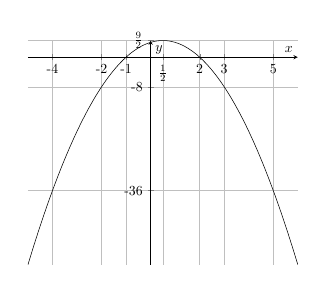
\begin{tikzpicture}[scale=0.5]
\begin{axis}[
    axis lines = middle,
    grid=major,
    legend pos={south west},
    xlabel = {$x$},
    %xlabel style={below right},
    ylabel = {$y$},
    xtick={-4, -2,-1,0.5,2, 3, 5},
    xticklabels={-4, -2,-1,$\frac{1}{2}$,2, 3,5},
    ytick={-36,-8,4.5},
    yticklabels={-36,-8,$\frac{9}{2}$},
               ]
	\addplot[domain=-5:6, samples=100, color=black] {-2*x*x+2*x+4};
%\addplot[domain=-3.1:2.5, samples=100, color=red] {70*abs(1-2*abs(abs(x)-2))-10*x^2+10*x-70};
	%\addlegendentry{$\text{Рис. 1}$};
\end{axis}
\end{tikzpicture}$$
